%<dscrpt>Suite de nombres complexes avec des comparaisons et développements de suites réelles.</dscrpt>
\begin{figure}[h]
  \centering
  \begin{minipage}{6cm}
    \centering
    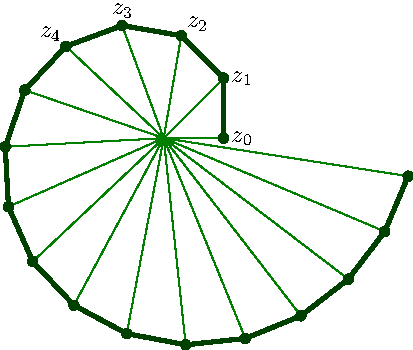
\includegraphics[width=4.5cm]{./ESpira_1.pdf}
    \caption{Définition des points $z_i$.}
    \label{fig:ESpira_1}
  \end{minipage}
  \begin{minipage}{6cm}
    \centering
    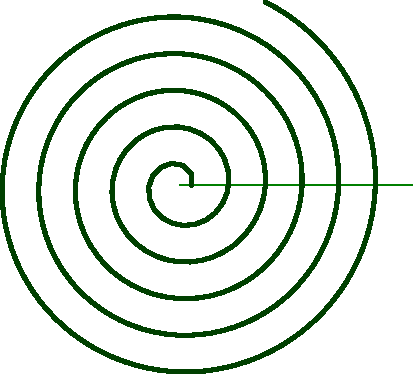
\includegraphics[width=4.5cm]{./ESpira_2.pdf}
    \caption{Intersection avec $]0,+\infty[$.}
    \label{fig:ESpira_2}
  \end{minipage}
\end{figure}
On définit par récurrence une suite $(z_n)_{n\in \N^*}$ de nombres complexes à l'aide de propriétés géométriques. Soit $O$ le point d'affixe $0$, fixons $z_{0}=1$ et construisons $z_{n}$ à partir de $z_{n-1}$ en imposant des conditions sur le triangle $Oz_{n-1}z_{n}$. Il doit être:
\begin{center}
  \emph{rectangle} en $ z_{n-1}$,
  \hspace{0.5cm} orient{\'e} \emph{dans le sens direct},
  \hspace{0.5cm} tel que $ |z_{n-1}- z_{n}|=1$.
\end{center}
La r{\'e}union des segments $[ z_{n},z_{n+1}]$ constitue une ligne polygonale infinie (notée $L$) de forme spirale (figures \ref{fig:ESpira_1} et \ref{fig:ESpira_2}).

\subsection*{Partie I. Expression d'un argument.}
\begin{enumerate}
\item Formuler très précisément un résultat de cours liant la fonction $\arctan$ avec un argument d'un nombre complexe non nul.
\item Exprimer $z_n$ en fonction de $z_{n-1}$ de $|z_{n-1}|$ et de $i$ puis $|z_{n+1}|$ en fonction de $z_n$. En déduire $|z_{n}|$ en fonction de $n$. 
\item Pour $n\geq 1$, on définit $\alpha_n$ par :
\[\alpha_{n}=\sum_{k=1}^{n}\arctan\frac{1}{\sqrt{k}}\]
Montrer que $\alpha_n$ est un argument de $ z_{n}$.
\end{enumerate}

\subsection*{Partie II. Lemme technique.}
Dans cette partie, $(u_n)_{n\geq 2}$ et $(v_n)_{n\geq 2}$ sont deux suites de r{\'e}els strictement positifs. On d{\'e}finit $(U_n)_{n\geq 2}$ et $(V_n)_{n\geq 2}$ par
\begin{displaymath}
 U_n =u_2+u_3+\cdots+u_n,\hspace{0.5cm} V_n =v_2+v_3+\cdots+v_n  
\end{displaymath}
\begin{enumerate}
\item Calculer un {\'e}quivalent de la forme $\frac{A}{n\sqrt{n}}$ ($A$ r{\'e}el) pour
\[\left(\frac{1}{\sqrt{n-1}}-\frac{1}{\sqrt{n}}\right)_{n\geq 2}\]
\item
On suppose $(u_n)_{n\geq 2}$ domin{\'e}e par $(v_n)_{n\geq 2}$ et $(V_n)_{n\geq 2}$ convergente vers un réel $V$.
\begin{enumerate}
\item Montrer que $(U_n)_{n\geq 2}$ est convergente. On note $U$ sa limite.
\item Montrer que $(U-U_n)_{n\geq 2}$ est domin{\'e}e par $(V-V_n)_{n\geq 2}$.
\end{enumerate}
\item Soit $B>0$ et $(u_n)_{n\geq 2}$ une suite {\'e}quivalente {\`a} $(Bn^{-\frac{3}{2}})_{n\geq 2}$. Montrer que $(U_n)_{n\geq 2}$ est convergente et que, si $U$ est sa limite, $(U-U_n)_{n\geq 2}$ est domin{\'e}e par $(n^{-\frac{1}{2}})_{n\geq 2}$.
\end{enumerate}

\subsection*{Partie III. Un développement asymptotique.}
Pour $n\geq1$, on pose
\begin{displaymath}
  u_n=2\sqrt n-2\sqrt {n-1}-\arctan \frac{1} {\sqrt n}
\end{displaymath}
\begin{enumerate}
\item Déterminer une suite simple {\'e}quivalente {\`a} $(u_n)_{n\in \N}$. En déduire que $(u_n)_{n\in \N}$ v{\'e}rifie les hypoth{\`e}ses de II.3.
\item \'Etablir l'existence d'une constante r{\'e}elle $C$ telle que
\begin{displaymath}
  \alpha_n=2\sqrt n-C+O(n^{-\frac{1}{2}})
\end{displaymath}
\end{enumerate}

\subsection*{Partie IV. Intersection avec $]0,+\infty[$.}
On parcourt la ligne polygonale $L$ dans le sens direct {\`a} partir de $z_0$.
\begin{enumerate}
\item Montrer que $L$ coupe la demi-droite $[0,+\infty]$ en une infinit{\'e} de points notés successivement $M_0(=z_0),M_1,\ldots,M_k,\ldots$ (figure \ref{fig:ESpira_2}). \newline
L'unique ar{\^e}te de la ligne polygonale $L$ qui contient le point $M_k$ ($k\geq 1$), est d{\'e}sign{\'e}e par $]z_{v(k)-1},z_{v(k)}]$.
\item Montrer que $v(k)\sim k^2 \pi^2$ en $+\infty$ et en déduire
\begin{displaymath}
v(k)=k^2\pi^2 + C\pi k + \frac{C^2}{4} + O(1)  
\end{displaymath}
\end{enumerate}
